\section{Лекция 4. Конусы}
\subsection{Определение}
\noindent\textbf{Определение 2.20}
Подмножество $K\subseteq \mathbb{R}^n$ является \textbf{конусом},\\
 когда $K\neq \varnothing$ и $\forall x\in K$ и $\alpha \geq 0$ выполняется $\alpha x \in K$.\\
 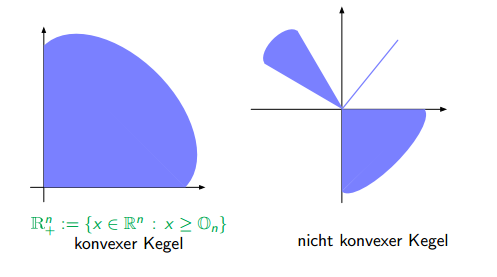
\includegraphics[scale=1]{kegel.png}
\subsection{Свойства конусов}
\noindent\textbf{Замечание 2.21}\\
Пусть $I$ является множеством индексов (произвольной мощности) и $K_{i}\subseteq \mathbb{R}^n$ - конусы ($i \in I$), тогда множество пересечений $\cap_{i \in I} K_{i}$ является конусом.\\

\noindent\textbf{Замечание 2.22}\\
Непустое множество $\varnothing \neq K \subseteq \mathbb{R}^n$ является выпуклым конусом тогда и только тогда, когда $K$ содержит все конические комбинации своих элементов.\\

\noindent$\blacktriangleleft$ Требуется показать, что $\forall x,y \in K, \forall \lambda,\mu >0$ : $\lambda x +\mu y \in K$\\
\begin{itemize}
\item В связи с выпуклостью $K$ имеем: $\displaystyle\frac{\lambda}{\lambda +\mu}x+ \frac{\mu}{\lambda +\mu}y \in K$
\item $\displaystyle z:=\frac{\lambda}{\lambda +\mu}x+ \frac{\mu}{\lambda +\mu}y$
\item Т.к. $K$ - конус $\Longrightarrow$ $\lambda x +\mu y=(\lambda +\mu)z \in K$. $\blacktriangleright$
\end{itemize}
\subsection{Важные примеры конусов}
\begin{itemize}
\item \textbf{Неотрицательный октант}
\begin{equation*}
\mathbb{R}^{n}_{+}:=\left\lbrace x \in \mathbb{R}^{n} | x \geq \mathbb{O}^{n} \right\rbrace
\end{equation*}
\item \textbf{Конус симметрических неотрицательно определенных матриц}
\begin{equation*}
\mathbb{S}^{k}_{+}:=\left\lbrace A \in \mathbb{S}^{k} | x^{T}Ax \geq 0, \forall x \in \mathbb{R}^{k}  \right\rbrace
\end{equation*}
$\blacktriangleleft$
$A,B \in \mathbb{S}^{k}_{+} \text{, } \lambda,\mu \geq 0 :
\text{\\ матрица } A$ положительно полуопределена, если
\begin{equation*}
\forall x \in \mathbb{R}^{k} : x^{T}Ax\geq 0
\end{equation*}
Коническая комбиначия симметрических матриц является симметрической матрицей:
\begin{equation*}
\Longrightarrow x^{T}\left(\lambda A + \mu B\right)x = x^{T}\lambda A x + x^{T}\mu B x \geq 0
\end{equation*}
$\Longrightarrow \mathbb{S}^{k}_{+}$ -- выпуклый конус. $\blacktriangleright$
\item $\mathbb{S}^{k}_{+} \text{ и } \mathbb{R}^{n}_{+}$ выпуклые и замкнутые множества.\\
\begin{equation*}
\blacktriangleleft \mathbb{S}^{k}_{+}=\left\lbrace A \in \mathbb{S}^{k} :  x^{T} A x \geq 0 \text{, } \forall x \in \mathbb{R}^{k}  \right\rbrace = \bigcap_{x \in \mathbb{R}^{k}} \left\lbrace A \in \mathbb{S}^{k} :  x^{T} A x \geq 0 \right\rbrace
\end{equation*}
Определим отображение $\varphi_{x}: \mathbb{S}^{k} \longrightarrow \mathbb{R} \text{ как } \varphi_{x} (A):= x^{T} A x$
Имеем: \begin{equation*}
\left\lbrace A \in \mathbb{S}^{k} :  x^{T} A x \geq 0 \right\rbrace = \varphi_{x}^{-1}\left(\left[ 0, \infty \right[ \right)
\end{equation*}
Множество $\left[ 0, \infty \right[ $ -- замкнуто, прообраз замкнутого -- замкнут, пересечение любого количества замкнутых множеств -- замкнуто.\\
$\Longrightarrow \mathbb{S}^{k}_{+}\text{-- замкнуто.}$
$\blacktriangleright$
\end{itemize}
\subsection{Теорема отделимости для выпуклых конусов}
\noindent\textbf{Теорема 2.23}\\
Пусть $K \subseteq \mathbb{R}^{n}$ есть замкнутый выпуклый конус и $y \in \mathbb{R}^{n} \ K$ - точка, находящаяся вне $K$, тогда есть $a \in \mathbb{R}^{n}$ что
\begin{center}
$\left\langle a,x \right\rangle \leq 0$ для любого $ x \in K $ и $ \left\langle a,y \right\rangle = 1 $
\end{center}
$\blacktriangleleft$
 \begin{equation} \label{one}
$$По \textbf{Теореме 2.15}$$ \Longrightarrow \exists a \in \mathbb{R}^{n} \setminus \left\lbrace\mathbb{O}_{n}\right\rbrace : \left\langle a,x \right\rangle < \left\langle a,y \right\rangle \forall x \in K
\end{equation}
Т.к. $ \mathbb{O}_{n} \in K$, то $\left\langle a,y \right\rangle >0$
\begin{equation} \label{two}
\text{При масштабировании: } \displaystyle\left( a \longleftarrow \frac{1}{\left\langle a,y \right\rangle}a \right) \text{ получим } \left\langle a,y \right\rangle = 1
\end{equation}
 Пусть сущестует $x \in K$ что $\left\langle a,x \right\rangle > 0$.
 По определению конуса $\forall \lambda >0$ $\lambda x \in K$ и $\left\langle a,\lambda x \right\rangle =\lambda \left\langle a,x \right\rangle$.\\
Получили противоречие с условиями (1) и (2), т.к. можно выбрать $\lambda >0$ при котором $\lambda \left\langle a,x \right\rangle > 1$. $\blacktriangleright$
\subsection{Конические оболочки}
\noindent\textbf{Определение 2.24}\\
Пусть $X \subseteq \mathbb{R}^{n}$. Конической оболочкой множества $X$ называют множество
\begin{equation*}
coneX:=\cap \left\lbrace K \subseteq \mathbb{R}^{n}|X \subseteq K, K \text{ -- конус} \right\rbrace
\end{equation*}

\noindent\textbf{Замечание 2.25}\\
\begin{equation*}
coneX=\left\lbrace \alpha x | x \in X, \alpha \geq 0 \right\rbrace\cup\left\lbrace \mathbb{O}^{n} \right\rbrace
\end{equation*}
\noindent\textbf{Замечание 2.26}\\
\begin{itemize}
\item Для любого $X \subseteq \mathbb{R}^{n}$ коническая оболочка $coneX$ является конусом.
\item Для любого выпуклого множества $X$ коническая оболочка $coneX$ является выпуклым консуом.
\end{itemize}
\subsection{Выпуклые конические оболочки}
\noindent\textbf{Определение 2.27}\\
Для $X \subseteq \mathbb{R}^{n}$ множество
\begin{equation*}
cconeX:=\cap \left\lbrace K \subseteq \mathbb{R}^{n} | X \subseteq K, K \text{ -- выпуклый конус} \right\rbrace
\end{equation*}
является выпуклой конической оболочкой множества $X$.\\

\noindent\textbf{Замечание 2.28}\\
Для любого $X \subseteq \mathbb{R}^{n}$ выпуклая коническая оболочка $ccone X$ ...
\begin{itemize}
\item является выпуклым конусом.
\item есть множество всех конических комбинаций элементов из $X$.
\end{itemize}
\subsection{Конечнопорожденные конусы}
\noindent\textbf{Определение 2.29}\\
Конус называют \textbf{конечнопорожденным} для конечного множества \\
$X \subseteq \mathbb{R}^{n}$, если он является выпуклой конической оболочкой данного множества
\begin{equation*}
cconeX=\left\lbrace \sum_{x\in X} \lambda_{x} x |\lambda_{x}\geq 0, \forall x\in X \right\rbrace
\end{equation*}
Если $X \subseteq \mathbb{R}^{n}$ ленейно-независимо, то $cconeX$ называют \textbf{смплициальным} конусом.\\

\noindent\textbf{Замечание 2.30}\\
Конечнопорожденный конус является выпуклым.
\subsection{Теорема Каратеодори}
\noindent\textbf{Теорема 2.31}\\
Пусть $X \subseteq \mathbb{R}^{n}$ и $x \in cconeX$, тогда есть линейно-независимое подмножество $X_{1} \subseteq X$, что $x\in cconeX_{1}$ (В частности $|X_{1}|\leq n$).\\

$\blacktriangleleft$ Выберем $X_{1} \subseteq X$ как минимальное по мощности подмножество $X$, что коэффициенты $\lambda_{y} \geq 0$ $(y \in X_{1})$ и $\displaystyle x=\sum_{y \in X_{1}} \lambda_{y} y$.\\
В частности $\lambda_{y} > 0$ $\forall y \in X_{1}$.\\
Предположим, что $X_{1}$ линейно-зависимо. Следовательно существует набор $\mu_{y} \in \mathbb{R}^{n}$ $(y \in X_{1})$, где не все $\mu_{y}$ равны нулю, и $\displaystyle\sum_{y \in X_{1}} \mu_{y} y = 0$\\
Смасштабируем $\mu_{y}$ так, чтобы
\begin{equation*}
\displaystyle max\left\lbrace \frac{\mu_{y}}{\lambda_{y} }: y \in X_{1}\right\rbrace = 1
\end{equation*}
Рассмотрим $\displaystyle x=\sum_{y \in X_{1}} \lambda_{y} y - \sum_{y \in X_{1}} \mu_{y} y =\sum_{y \in X_{1}} \left(\lambda_{y}-\mu_{y}\right) y$\\
В сумме $\sum_{y \in X_{1}} \left(\lambda_{y}-\mu_{y}\right) y$ присутствует на один вектор меньше, чем в изначальной. Получили противоречие с выбором минимальности $X_{1}$. $\blacktriangleright$\\

\noindent\textbf{Теорема 2.32}\\
Конечнопорожденный конус является выпуклым и замкнутым.\\
$\blacktriangleleft$
\begin{itemize}
\item Пусть $X \subseteq \mathbb{R}^{n} \text{, } |X|< \infty \text{, } K:=ccone(X)$.
\item $K$, очевидно, выпукло.
\item По теореме 2.31 $\displaystyle\Longrightarrow \text{ } ccone(X)= \bigcup_{\hat{X}\subseteq X} \text{ } ccone(\hat{X}) \text{, где } \hat{X} \subseteq X \text{, } \hat{X}$-- линейно-независимы.
\item Т.к. конечное объединение замкнутых множеств - замкнуто, достаточно показать, что для каждого линейно-независимого подмножества $\hat{X} \subseteq \mathbb{R}^{n}$ симплициальный конус $ccone(\hat{X})$ замкнут.
\item Дополним $\hat{X}$ до базиса из $\mathbb{R}^{n}$ как  $\hat{X} \sqcup Y$ и определим линейное отображение $\varphi \text{: } \mathbb{R}^{n} \longrightarrow \mathbb{R}^{\hat{X}} \text{ как } \varphi \left( x \right):=\mathbbm{e_{x}} \text{, } \forall x \in \hat{X}$ и $\varphi \left( y \right):= \mathbb{O} \text{, } \forall y \in Y$
\item Прообраз $\varphi^{-1}\left( \mathbb{R}^{\hat{X}}_{+}\right)$ множества $\mathbb{R}^{\hat{X}}_{+}$ замкнуто, т.к. $\varphi$ непрерывно и $\mathbb{R}^{\hat{X}}_{+}$ замкнуто.
\item $\varphi^{-1}\left( \mathbb{R}^{\hat{X}}_{+} \right)=\left\lbrace \displaystyle\sum_{x \in \hat{X}} \lambda_{x} x + \sum_{y \in Y} \mu_{y} y  \text{ :} \lambda_{x} \geq 0 \text{, } \forall x \in \hat{X} \text{, } \mu_{y} \in \mathbb{R} \text{, } \forall y \in Y \right\rbrace = \displaystyle ccone(\hat{X}) +lin(Y)$
\item Т.к. $lin(\hat{X})\cap lin(Y)= \left\lbrace \mathbb{O} \right\rbrace \text{ :} \varphi^{-1}\left( \mathbb{R}^{\hat{X}}_{+} \right) \cap lin(\hat{X})=ccone(\hat{X})$. Множества $\varphi^{-1}\left( \mathbb{R}^{\hat{X}}_{+} \right) \text{ - замкнуто и } lin(\hat{X})$ - замкнуто.
\item $\Longrightarrow ccone(\hat{X})$ - замкнуто. $\blacktriangleright$
\end{itemize}
